% Options for packages loaded elsewhere
\PassOptionsToPackage{unicode}{hyperref}
\PassOptionsToPackage{hyphens}{url}
\PassOptionsToPackage{dvipsnames,svgnames,x11names}{xcolor}
%
\documentclass[
  12pt,
  a4paper]{article}
\usepackage{amsmath,amssymb}
\usepackage{lmodern}
\usepackage{iftex}
\ifPDFTeX
  \usepackage[T1]{fontenc}
  \usepackage[utf8]{inputenc}
  \usepackage{textcomp} % provide euro and other symbols
\else % if luatex or xetex
  \usepackage{unicode-math}
  \defaultfontfeatures{Scale=MatchLowercase}
  \defaultfontfeatures[\rmfamily]{Ligatures=TeX,Scale=1}
\fi
% Use upquote if available, for straight quotes in verbatim environments
\IfFileExists{upquote.sty}{\usepackage{upquote}}{}
\IfFileExists{microtype.sty}{% use microtype if available
  \usepackage[]{microtype}
  \UseMicrotypeSet[protrusion]{basicmath} % disable protrusion for tt fonts
}{}
\makeatletter
\@ifundefined{KOMAClassName}{% if non-KOMA class
  \IfFileExists{parskip.sty}{%
    \usepackage{parskip}
  }{% else
    \setlength{\parindent}{0pt}
    \setlength{\parskip}{6pt plus 2pt minus 1pt}}
}{% if KOMA class
  \KOMAoptions{parskip=half}}
\makeatother
\usepackage{xcolor}
\IfFileExists{xurl.sty}{\usepackage{xurl}}{} % add URL line breaks if available
\IfFileExists{bookmark.sty}{\usepackage{bookmark}}{\usepackage{hyperref}}
\hypersetup{
  pdftitle={Example},
  pdfauthor={Emma Cliffe},
  colorlinks=true,
  linkcolor={blue},
  filecolor={Maroon},
  citecolor={Blue},
  urlcolor={Blue},
  pdfcreator={LaTeX via pandoc}}
\urlstyle{same} % disable monospaced font for URLs
\usepackage[margin=2.5cm]{geometry}
\usepackage{graphicx}
\makeatletter
\def\maxwidth{\ifdim\Gin@nat@width>\linewidth\linewidth\else\Gin@nat@width\fi}
\def\maxheight{\ifdim\Gin@nat@height>\textheight\textheight\else\Gin@nat@height\fi}
\makeatother
% Scale images if necessary, so that they will not overflow the page
% margins by default, and it is still possible to overwrite the defaults
% using explicit options in \includegraphics[width, height, ...]{}
\setkeys{Gin}{width=\maxwidth,height=\maxheight,keepaspectratio}
% Set default figure placement to htbp
\makeatletter
\def\fps@figure{htbp}
\makeatother
\setlength{\emergencystretch}{3em} % prevent overfull lines
\providecommand{\tightlist}{%
  \setlength{\itemsep}{0pt}\setlength{\parskip}{0pt}}
\setcounter{secnumdepth}{-\maxdimen} % remove section numbering

\ifLuaTeX
  \usepackage{selnolig}  % disable illegal ligatures
\fi

\title{Example}
\author{Emma Cliffe}
\date{2022}

\begin{document}
\maketitle

{
\hypersetup{linkcolor=}
\setcounter{tocdepth}{2}
\tableofcontents
}
\hypertarget{alternative-formats}{%
\section{Alternative formats}\label{alternative-formats}}

It is recommended that you \href{./arclengthInR.html}{read this resource
on the web} but you can also download \href{./arclengthInR.pdf}{this
resource as a PDF} or download \href{./arclengthInR.docx}{this resource
as a Word document}.

\hypertarget{arc-length}{%
\section{Arc length}\label{arc-length}}

We often need to know the length of a curve between two points,
e.g.~what is the length of the ropes holding Clifton suspension bridge
(see Exercise Sheet 3).

\hypertarget{visualisation}{%
\subsection{Visualisation}\label{visualisation}}

Given a curve \(y=y(x)\)

\centering

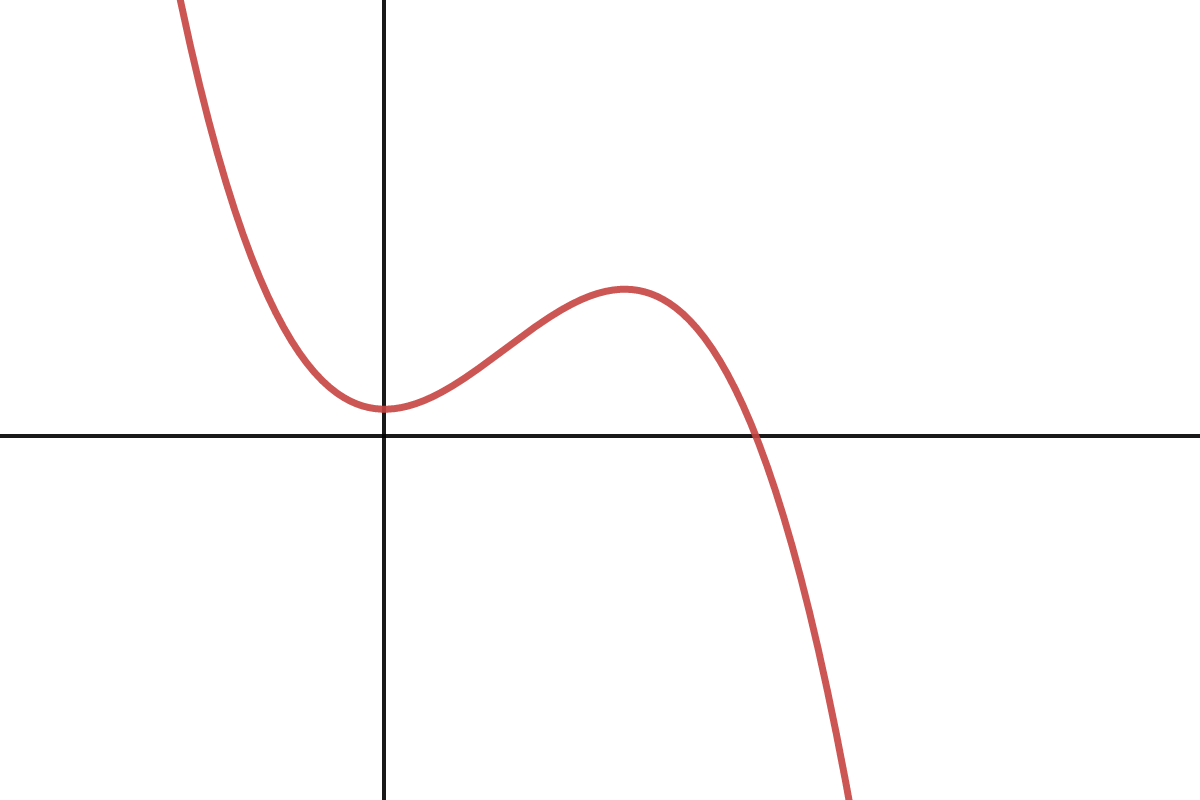
\includegraphics[height=0.2\textheight]{arclength1}

\flushleft

Accessible interactive graph at
\url{https://www.desmos.com/calculator/t8dz6vlmnz}

Let \(S\) be the arc length and \(\Delta S\) a short section of it.

\centering

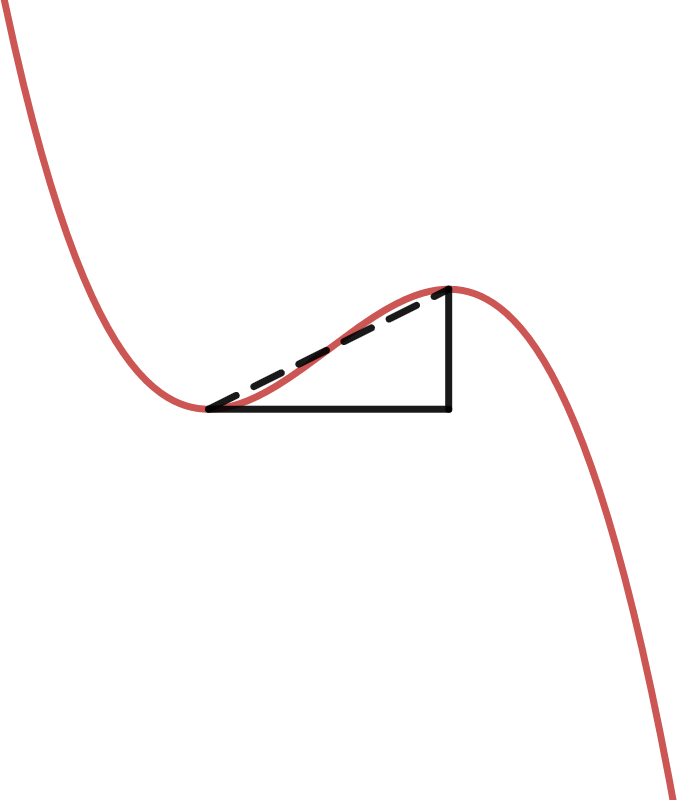
\includegraphics[height=0.2\textheight]{arclengthdx}

\flushleft

Accessible interactive graph at
\url{https://www.desmos.com/calculator/g5duc4kmfp}

\hypertarget{derivation-of-arc-length}{%
\subsection{Derivation of Arc Length}\label{derivation-of-arc-length}}

By Pythagoras' Theorem, \[
\Delta S^2 \approx \Delta x^2+\Delta y^2
\qquad \Rightarrow\qquad
\left(\dfrac{\Delta S}{\Delta x}\right)^2 \approx 1+\left(\dfrac{\Delta y}{\Delta x}\right)^2
\] As \(\Delta x\to0\) this becomes an identity \[
\left(\dfrac{dS}{dx}\right)^2 = 1+\left(\dfrac{dy}{dx}\right)^2
\qquad\Rightarrow\qquad
\dfrac{dS}{dx} = \sqrt{1+\left(\dfrac{dy}{dx}\right)^2}
\] The arclength between \(x=a\) and \(x=b\) is then \[
\begin{aligned}
  S(a,b) &= \int_a^b\dfrac{dS}{dx}dx\\
  &= \int_a^b\sqrt{1+\left(\dfrac{dy}{dx}\right)^2}dx.
\end{aligned}
\]

\end{document}
